\documentclass[11pt,openany]{article}

\usepackage{mathtools, commath}
% Packages for formatting
\usepackage[margin=1in]{geometry}
\usepackage{fancyhdr}
\usepackage{enumerate}
\usepackage{graphicx}
\usepackage{kotex}
\usepackage{arydshln} % Include this package
\usepackage{bbding}
\usepackage{amsmath}
\usepackage{amsthm}
\usepackage[dvipsnames,table]{xcolor}
\usepackage{amssymb, amsfonts}
\usepackage{wasysym}
\usepackage{footnote}
\usepackage{tablefootnote}
\usepackage{arydshln} % Include this package
% Fonts
\usepackage[T1]{fontenc}
\usepackage[utf8]{inputenc}
\usepackage{newpxtext,newpxmath}
\usepackage{sectsty}

% Define colors
\definecolor{TealBlue1}{HTML}{0077c2}
\definecolor{TealBlue2}{HTML}{00a5e6}
\definecolor{TealBlue3}{HTML}{b3e0ff}
\definecolor{TealBlue4}{HTML}{00293c}
\definecolor{TealBlue5}{HTML}{e6f7ff}

\definecolor{thmcolor}{RGB}{231, 76, 60}
\definecolor{defcolor}{RGB}{52, 152, 219}
\definecolor{lemcolor}{RGB}{155, 89, 182}
\definecolor{corcolor}{RGB}{46, 204, 113}
\definecolor{procolor}{RGB}{241, 196, 15}

\usepackage{color,soul}
\usepackage{soul}
\newcommand{\mathcolorbox}[2]{\colorbox{#1}{$\displaystyle #2$}}
\usepackage{cancel}
\newcommand\crossout[3][black]{\renewcommand\CancelColor{\color{#1}}\cancelto{#2}{#3}}
\newcommand\ncrossout[2][black]{\renewcommand\CancelColor{\color{#1}}\cancel{#2}}

\usepackage{hyperref}
\usepackage{booktabs}

% Chapter formatting
\definecolor{titleTealBlue}{RGB}{0,53,128}
\usepackage{titlesec}
\titleformat{\section}
{\normalfont\sffamily\Large\bfseries\color{titleTealBlue!100!gray}}{\thesection}{1em}{}
\titleformat{\subsection}
{\normalfont\sffamily\large\bfseries\color{titleTealBlue!50!gray}}{\thesubsection}{1em}{}

%Tcolorbox
\usepackage[most]{tcolorbox}
\usepackage{multirow}
\usepackage{multicol}

\usepackage[linesnumbered,ruled]{algorithm2e}
\usepackage{algpseudocode}
\usepackage{setspace}
\SetKwComment{Comment}{/* }{ */}
\SetKwProg{Fn}{Function}{:}{end}
\SetKw{End}{end}
\SetKw{DownTo}{downto}

% Define a new environment for algorithms without line numbers
\newenvironment{algorithm2}[1][]{
	% Save the current state of the algorithm counter
	\newcounter{tempCounter}
	\setcounter{tempCounter}{\value{algocf}}
	% redefine the algorithm numbering (remove prefix)
	\renewcommand{\thealgocf}{}
	\begin{algorithm}
	}{
	\end{algorithm}
	% Restore the algorithm counter state
	\setcounter{algocf}{\value{tempCounter}}
}

\usepackage{adjustbox}
% Header and footer formatting
\pagestyle{fancy}
\fancyhead{}
\fancyhf{}
\rhead{\textcolor{TealBlue2}{\large\textbf{기대수(기초부터 대학원 수학까지 시리즈) 3기}}}%\rule{3cm}{0.4pt}}
\lhead{\textcolor{TealBlue2}{\large\textbf{수학의 즐거움, Enjoying Math}}}
% Define footer
%\newcommand{\footer}[1]{
%\begin{flushright}
%	\vspace{2em}
%	\includegraphics[width=2.5cm]{school_logo.jpg} \\
%	\vspace{1em}
%	\textcolor{TealBlue2}{\small\textbf{#1}}
%\end{flushright}
%}
%\rfoot{\large Department of Information Security, Cryptogrphy and Mathematics, Kookmin Uni.\includegraphics[height=1.5cm]{school_logo.jpg}}
\fancyfoot{}
\fancyfoot[C]{-\thepage-}

\usepackage{tcolorbox}
\tcbset{colback=white, arc=5pt}

\definecolor{axiomcolor}{HTML}{a88bfa}
\definecolor{defcolor}{RGB}{52, 152, 219}
\definecolor{procolor}{RGB}{241, 196, 15}
\definecolor{thmcolor}{RGB}{231, 76, 60}
\definecolor{lemcolor}{RGB}{155, 89, 182}
\definecolor{corcolor}{RGB}{46, 204, 113}
\definecolor{execolor}{RGB}{90, 128, 127}

% Define a new command for the custom tcolorbox
\newcommand{\axiombox}[2][]{%
	\begin{tcolorbox}[colframe=axiomcolor, title={\color{white}\bfseries #1}]
		#2
	\end{tcolorbox}
}

\newcommand{\defbox}[2][]{%
	\begin{tcolorbox}[colframe=defcolor, title={\color{white}\bfseries #1}]
		#2
	\end{tcolorbox}
}

\newcommand{\lembox}[2][]{%
	\begin{tcolorbox}[colframe=lemcolor, title={\color{white}\bfseries #1}]
		#2
	\end{tcolorbox}
}

\newcommand{\probox}[2][]{%
	\begin{tcolorbox}[colframe=procolor, title={\color{white}\bfseries #1}]
		#2
	\end{tcolorbox}
}

\newcommand{\thmbox}[2][]{%
	\begin{tcolorbox}[colframe=thmcolor, title={\color{white}\bfseries #1}]
		#2
	\end{tcolorbox}
}

\newcommand{\corbox}[2][]{%
	\begin{tcolorbox}[colframe=corcolor, title={\color{white}\bfseries #1}]
		#2
	\end{tcolorbox}
}



\usepackage{amsthm}

% Define custom theorem styles
\newtheoremstyle{dotless} % Name of the style
{3pt} % Space above
{3pt} % Space below
{\itshape} % Body font
{} % Indent amount
{\bfseries} % Theorem head font
{} % Punctuation after theorem head
{2.5mm} % Space after theorem head
{} % Theorem head spec

\newtheoremstyle{definitionstyle} % Name of the style
{3pt} % Space above
{3pt} % Space below
{} % Body font
{} % Indent amount
{\bfseries} % Theorem head font
{.} % Punctuation after theorem head
{2.5mm} % Space after theorem head
{} % Theorem head spec

% Applying custom styles
\theoremstyle{dotless}
\newtheorem{theorem}{Theorem} % Theorem environment with section-wise numbering
\newtheorem{proposition}[theorem]{Proposition} % Theorem environment with section-wise numbering
\newtheorem{lemma}[theorem]{Lemma} % Lemma shares the counter with theorem
\newtheorem{corollary}[theorem]{Corollary} % Corollary shares the counter with theorem

\theoremstyle{definitionstyle}
\newtheorem*{observation}{\textcolor{Magenta}{Observation}}
\newtheorem{definition}{Definition} % Definition shares the counter with theorem
\newtheorem{example}{Example} % Example shares the counter with theorem
\newtheorem{exercise}{Exercise} % Example shares the counter with theorem
\newtheorem{remark}{Remark} % Remark shares the counter with theorem
\newtheorem*{note}{Note}

\newtheorem*{definition*}{Definition} % Definition shares the counter with theorem
\newtheorem*{example*}{Example} % Example shares the counter with theorem
\newtheorem*{exercise*}{\textcolor{violet}{Exercise}} % Example shares the counter with theorem
\newtheorem*{remark*}{Remark} % Remark shares the counter with theorem


\usepackage{tikz}
\usepackage{tikz-cd}
\usepackage{tikz-3dplot}
\usepackage{pgfplots}
\pgfplotsset{compat=newest} % Adjust to your version of pgfplots
\def\Circlearrowleft{\ensuremath{%
		\rotatebox[origin=c]{180}{$\circlearrowleft$}}}
\def\Circlearrowright{\ensuremath{%
		\rotatebox[origin=c]{180}{$\circlearrowright$}}}
\def\CircleArrowleft{\ensuremath{%
		\reflectbox{\rotatebox[origin=c]{180}{$\circlearrowleft$}}}}
\def\CircleArrowright{\ensuremath{%
		\reflectbox{\rotatebox[origin=c]{180}{$\circlearrowright$}}}}
\usetikzlibrary{
	3d, % For 3D drawing
	angles,
	arrows,
	arrows.meta,
	backgrounds,
	bending,
	calc,
	decorations.pathmorphing,
	decorations.pathreplacing,
	decorations.markings,
	fit,
	matrix,
	patterns,
	patterns.meta,
	positioning,
	quotes,
	shadows,
	shapes,
	shapes.geometric,
	tikzmark
}
\tikzset{
	% single mid‐path arrow
	mid arrow/.style={
		decoration={
			markings,
			mark=at position 0.5 with {\arrow{Stealth[scale=1.2]}}
		},
		postaction={decorate},
	},
	% style for field arrows
	field arrow/.style={
		-{Stealth[scale=1.0]},
		thick,
		blue!70!black,
	},
}
\newcommand{\ie}{\textnormal{i.e.}}
\newcommand{\rsa}{\mathsf{RSA}}
\newcommand{\rsacrt}{\mathsf{RSA}\textendash\mathsf{CRT}}
\newcommand{\inv}[1]{#1^{-1}}

%New Command
%\newcommand{\set}[1]{\left\{#1\right\}}
\newcommand{\N}{\mathbb{N}}
\newcommand{\Z}{\mathbb{Z}}
\newcommand{\Q}{\mathbb{Q}}
\newcommand{\R}{\mathbb{R}}
\newcommand{\cR}{\mathcal{R}}
\newcommand{\C}{\mathbb{C}}
\newcommand{\F}{\mathbb{F}}
\newcommand{\nbhd}{\mathcal{N}}
\newcommand{\Log}{\operatorname{Log}}
\newcommand{\Arg}{\operatorname{Arg}}
\newcommand{\pv}{\operatorname{P.V.}}

\newcommand{\of}[1]{\left( #1 \right)} 
%\newcommand{\abs}[1]{\left\lvert #1 \right\rvert}
%\newcommand{\norm}[1]{\left\| #1 \right\|}

\newcommand{\sol}{\textcolor{magenta}{\bf Sol}}
\newcommand{\conjugate}[1]{\overline{#1}}

\newcommand{\res}{\operatorname{res}}
\DeclareMathOperator*{\Res}{\operatorname{Res}}

%\renewcommand{\Re}{\operatorname{Re}}
%\renewcommand{\Im}{\operatorname{Im}}

\newcommand{\cyclic}[1]{\langle #1 \rangle}
\newcommand{\uniform}{\overset{\$}{\leftarrow}}
\newcommand{\xmark}{\textcolor{red}{\XSolidBrush}}
\newcommand{\vmark}{\textcolor{green!75!black}{\CheckmarkBold}}

\newcommand{\gen}[1]{\langle #1 \rangle}
\newcommand{\Gen}[1]{\left\langle #1 \right\rangle}

\newcommand{\img}[1]{\text{Img}(#1)}
\newcommand{\Img}[1]{\text{Img}\left(#1\right)}
\newcommand{\preimg}[1]{\text{Img}^{-1}(#1)}
\newcommand{\Preimg}[1]{\text{Img}^{-1}\left(#1\right)}

\newcommand{\relation}{\mathrel{\mathcal{R}}}
\newcommand{\injection}{\rightarrowtail}
\newcommand{\surjection}{\twoheadrightarrow}
\newcommand{\id}{\textnormal{id}}

\newcommand{\eqclass}[1]{\left[#1\right]}

% Define custom colors for O and X
\newcommand{\yes}{\textcolor{blue}{\bf \fullmoon}}
\newcommand{\no}{\textcolor{red}{\bf \texttimes}}

\DeclarePairedDelimiter\ceil{\lceil}{\rceil}
\DeclarePairedDelimiter\floor{\lfloor}{\rfloor}
%\renewcommand{\floor}[#1]{\lfloor #1\rfloor}
%\newcommand{\Floor}[#1]{\left\lfloor #1\right\rfloor}
%\newcommand{\ceil}[#1]{\lceil #1\rceil}
%\newcommand{\Ceil}[#1]{\left\lceil #1\right\rceil}

\newcommand{\topology}{\mathscr{T}}
\newcommand{\sequence}[1]{\langle #1\rangle}

\setstretch{1.25}
\begin{document}
\pagenumbering{arabic}
\begin{center}
	\huge\textbf{Set Theory I}\\
	\vspace{0.5em}
	\large{Ji, Yong-hyeon}\\
	\vspace{0.5em}
	\normalsize{\today}\\
\end{center}

\paragraph*{Terminology.}

\begin{itemize}
	\item Set; Collection; Family.
	\item Tabular (or Roster) Form \[
	A=\set{0,2,4,8}.
	\]
	\item Set-builder Form \[
	A=\set{x:x\ \text{is even and}\ x <10}.
	\]
\end{itemize}

\begin{example*}
	\ \begin{itemize}
		\item $\mathbb{N}=\set{1,2,\dots}$
		\item $\mathbb{Z}=\set{\dots,-2,-1,0,1,2,\dots}$
		\item $\mathbb{Q}=\set{\frac{p}{q}:p\in\mathbb{Z},q\in\mathbb{Z}\setminus\set{0}, \gcd(p,q)=1}$
		\item $\mathbb{R}=\set{x: x\ \text{is a real number}}$
		\item $\mathbb{C}=\set{z:z\ \text{is a complex number}}$
	\end{itemize}
\end{example*}
\vfill
\begin{exercise*}
	Show that $\sqrt{2}$ is irrational.
	\begin{proof}[\sol]
		\textcolor{gray!30!white}{Assume \( \sqrt{2} \in \mathbb{Q} \), i.e., \( \exists p, q \in \mathbb{Z} \) such that
		$\sqrt{2}q = p, \quad g\neq 0$ and $\gcd(p, q) = 1.$
		Then $2q^2 = p^2$. Since \( p^2 \) is even \( \Rightarrow p \) is even,
		\[
		p = 2k \quad \text{for some } k \in \mathbb{Z}
		\]
		By substituting \( p = 2k \) into \( 2q^2 = p^2 \), we have
		\[
		2q^2 = (2k)^2 \implies 2q^2 = 4k^2 \implies q^2 = 2k^2
		\]
		Since \( q^2 \) is even \( \Rightarrow q \) is even,
		\[
		q = 2m \quad \text{for some } m \in \mathbb{Z}
		\]
		Thus, \( p \) and \( q \) are both even \( \implies \gcd(p, q) \geq 2 \), which contradicts the assumption \( \gcd(p, q) = 1 \).}
	\end{proof}
\end{exercise*}

\newpage
\defbox[Subset and Set Equality]{\begin{definition*}
		Let $A$ and $B$ are sets.
		\begin{itemize}
			\item Subset: $
			B\subseteq A\overset{\text{def}}{\iff}(x\in B\Rightarrow x\in A).$
			\item Set Equality: \begin{align*}
				A=B&\overset{\text{def}}{\iff} A\subseteq B\land B\subseteq A\\
				&\iff (x\in A\Rightarrow x\in B)\land(x\in B\Rightarrow x\in A).
			\end{align*}
		\end{itemize}
\end{definition*}}
\vfill
\defbox[Power Set]{\begin{definition*}
	The \hl{\textbf{power set}} of a set $X$ is the set of all subsets of $X$.	
	\[
	\mathcal{P}(X)=2^X:=\set{S:S\subseteq X}.
	\]
\end{definition*}}
\vfill
\defbox[Cartesian Product]{\begin{definition*}
	Let $A$ and $B$ are sets. The \hl{\textbf{cartesian product}} of $A$ and $B$ is the set \[
	A\times B=\set{(a,b):a\in A\land b\in B}.
	\]
\end{definition*}}
\vfill
\defbox[Union, Intersection and Complement]{\begin{definition*}
	Let $U$ is a universal set, and let $A,B\subseteq U$.
	\begin{itemize}
		\item The \hl{\textbf{union}} of $A$ and $B$ is the set \[
		\boxed{A\cup B:=\set{x\in U:x\in A\lor x\in B}}.
		\] Note that $x\in A\cup B\iff x\in A\lor x\in B$.
		\item The \hl{\textbf{intersection}} of $A$ and $B$ is the set \[
		\boxed{A\cap B:=\set{x\in U:x\in A\land x\in B}}.
		\] Note that $x\in A\cap B\iff x\in A\land x\in B$.
		\item The \hl{\textbf{complement}} of $A$ is the set \[
		\boxed{A^C:=\set{x\in U:\lnot(x\in A)}=\set{x:x\notin A}}.
		\] Note that $x\in A^C\iff x\notin A$.
	\end{itemize}
\end{definition*}}

\newpage

\probox[]{\begin{proposition}
	Let $A,B,C\subseteq U$.
	\begin{enumerate}[(1)]
		\item $A\cap(B\cup C)=(A\cap B)\cup(A\cap C)$.
		\item $A\cup(B\cap C)=(A\cup B)\cap(A\cup C)$.
		\item $(A\cup B)^C=A^C\cap B^C$.
		\item $(A\cap B)^C=A^C\cup B^C$.
	\end{enumerate}
\end{proposition}}
\begin{proof}
	\begin{enumerate}[(1)]
		\item Refer to the Video\cite{set_thery_a}.
		\item Refer to the Video\cite{set_thery_a}.
		\item \textcolor{gray!30!white}{$(A\cup B)^C=\set{x:\lnot\left[x\in A\lor x\in B\right]}=\set{x:x\notin A\land x\notin B}=A^C\cap B^C.$}
		\item \textcolor{gray!30!white}{$(A\cap B)^C=\set{x:\lnot\left[x\in A\land x\in B\right]}=\set{x:x\notin A\lor x\notin B}=A^C\cup B^C.$}
	\end{enumerate}
\end{proof}

\vfill
\begin{exercise*}
	Let $A$ has $n$ elements. Show that $\mathcal{P}(A)$ has $2^n$ elements.
	\begin{proof}[\sol] 
		\textcolor{gray!30!white}{\begin{itemize}
			\item[(pf 1)] For each element of $A$, there are two choices:
			\begin{enumerate}
				\item Include the element in the subset.
				\item Exclude the element from the subset.
			\end{enumerate}
			Since we have two independent choices (include or exclude), the total number of subsets is:
			\[
			\underbrace{2\times 2\times\cdots 2}_{n\ \text{times}}=2^n.
			\]
			\item[(pf 2)] We use mathematical induction.
			\ \\
			(Basic Step) Let $A=\varnothing$ (so $\abs{A}=0$). Then $\mathcal{P}(A)=\set{\varnothing}$ and so $\abs{\mathcal{P}(A)}=\abs{\set{\varnothing}}=1$.
			\ \\
			(Inductive Step) Assume that $\abs{\mathcal{P}(A)}=2^k$ where $\abs{A}=k$ for some $k\in\mathbb{Z}_{\geq  0}$. Let $A'=A\cup\set{x}$ where $\abs{A}=k$ and $x\notin A$. That is, $\abs{A'}=k+1$. Then \[
			\mathcal{P}(A')=\mathcal{P}(A)\cup\set{S\cup \set{x}:S\in \mathcal{P}(A)}.
			\] This implies $\abs{\mathcal{P}(A')}=\abs{\mathcal{P}(A)} + \abs{\mathcal{P}(A)}.$ Therefore, by assumption, $\abs{\mathcal{P}(A')}=2^k + 2^k=2^{k+1}.$
		\end{itemize}}
	\end{proof}
\end{exercise*}

%\begin{note}[Mathematical Induction]
%	\ \begin{tcolorbox}[colback=white]
%		Let $S\subseteq\mathbb{N}$. If \begin{enumerate}[(1)]
%			\item $\min S=1\in S$,
%			\item $a\in S\implies a+1\in S$,
%		\end{enumerate} then $S=\mathbb{N}$.
%	\end{tcolorbox}
%\end{note}

\newpage
\defbox[Function]{\begin{definition*}
	Let $A$ and $B$ are sets. A relation $f\subseteq A\times B$ is a \hl{\textbf{function}} \textbf{from $\boldmath{A}$ to $\boldmath{B}$} if \[
	\boxed{\forall a\in A,\ \exists! b\in B\ \text{such that}\ (a,b)\in f.}
	\] That is, every element of $A$ relates to \underline{exactly one} element of $B$.
\end{definition*}}
\begin{remark*}
	\ \begin{itemize}
		\item The \hl{\textbf{domain}} of $f$ is $\text{Dom}(f)=A$.
		\item The \hl{\textbf{codomain}} of $f$ is $\text{Cdm}(f)=B$.
		\item The \hl{\textbf{image}} \textbf{of $A$ under $f$} is the set \begin{align*}\
			\img{f}=f[A]:&=\set{b\in B:\exists a \in A\ \text{s.t.}\ (a,b)\in f}\\
			&=\set{b\in B:\exists a \in A\ \text{s.t.}\ f(a)=b}\\
			&=\set{b\in B: b = f(a)\ \text{for at least one}\ a\in A}.
		\end{align*} Simply we can express it as $f[A]=\set{f(a)\in B:a\in A}$. 
		\begin{figure}[h!]\centering
			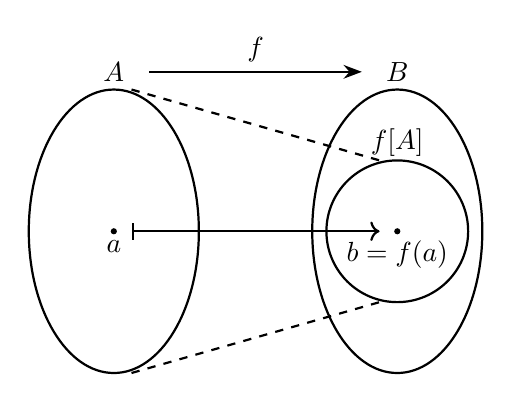
\begin{tikzpicture}[scale=.9]
	% Draw the sets A and B
	\draw[thick] (-2,0) ellipse (1.2 and 2);
	\draw[thick] (2,0) ellipse (1.2 and 2);
	\draw[thick] (2,0) ellipse (1 and 1);
	
	% Labels for sets
	\node at (-2, 2.25) {$A$};
	\node at (2, 2.25) {$B$};
	
	% Draw the arrows representing the function
	\draw[-Stealth, thick] (-1.5, 2.25) -- (1.5,2.25) node[midway, above] {$f$};
	
	\node at (2, 1.25) {$f[A]$};
	\draw[dashed, thick] (-1.75, 2) -- (1.75, 1);
	\draw[dashed, thick] (-1.75, -2) -- (1.75, -1);
	
	\filldraw (-2,0) circle (1pt) node[below] {$a$};
	\filldraw (2,0) circle (1pt) node[below] {$b=f(a)$};
	\draw[|->, thick] (-1.75, 0) -- (1.75, 0);
\end{tikzpicture}

			\caption{Image of $A$ under $f$.}
		\end{figure}\\
		Note that $f[A]\subseteq B=\text{Cdm}(f)$ and that \begin{align*}
			b\in f[A]\iff b=f(a)\ \text{for some}\ a\in A.
		\end{align*}
		\item The \hl{\textbf{preimage}} \textbf{of $B_1\subseteq B$ under $f$} is the set \begin{align*}
			f^{-1}[B_1]:&=\set{a\in A:\exists b \in B_1\ \text{s.t.}\ (a,b)\in f}\\
			&=\set{a\in A:\exists! b \in B_1\ \text{s.t.}\ b=f(a)}\ \text{by def. of a function}\\
			&=\set{a\in A:f(a)=b\ \text{for exactly one}\ b\in B_1}.
		\end{align*} ``Exactly one'' ensures a unique assignment for every element of $A$, while ``at most one'' allows no assignment. Simply we can express it as $f^{-1}[B_1]=\set{a\in A:f(a)\in B_1}$.
		\begin{figure}[h!]\centering
			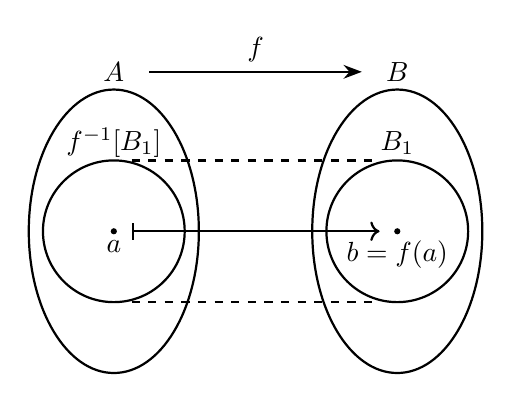
\begin{tikzpicture}[scale=.9]
	% Draw the sets A and B
	\draw[thick] (-2,0) ellipse (1.2 and 2);
	\draw[thick] (2,0) ellipse (1.2 and 2);
	\draw[thick] (-2,0) ellipse (1 and 1);
	\draw[thick] (2,0) ellipse (1 and 1);
	
	% Labels for sets
	\node at (-2, 2.25) {$A$};
	\node at (2, 2.25) {$B$};
	
	% Draw the arrows representing the function
	\draw[-Stealth, thick] (-1.5, 2.25) -- (1.5,2.25) node[midway, above] {$f$};
	
	\node at (2, 1.25) {$B_1$};
	\node at (-2, 1.25) {$f^{-1}[B_1]$};
	\draw[dashed, thick] (-1.75, 1) -- (1.75, 1);
	\draw[dashed, thick] (-1.75, -1) -- (1.75, -1);
	
	\filldraw (-2,0) circle (1pt) node[below] {$a$};
	\filldraw (2,0) circle (1pt) node[below] {$b=f(a)$};
	\draw[|->, thick] (-1.75, 0) -- (1.75, 0);
\end{tikzpicture}

			\caption{Preimage of $B_1\subseteq B$ under $f$.}
		\end{figure}\\
		Note that $f^{-1}[B_1]\subseteq A=\text{Dom}(f)$ and that $a\in f^{-1}[B_1]\iff f(a)\in B_1.$
	\end{itemize}
\end{remark*}

\vfill
\probox{\begin{proposition}
	Let $f:A\to B$ be a function from $A$ to $B$, and let $A_1,A_2\subseteq A$. \begin{enumerate}[(1)]
		\item $f[A_1\cup A_2]=f[A_1]\cup f[A_2]$.
		\item $f[A_1\cap A_2]\subseteq f[A_1]\cap f[A_2]$.
	\end{enumerate}
\end{proposition}}
\begin{proof}
\ \textcolor{gray!30!white}
%\ \textcolor{black}
{Recall that \[
	b\in f[A]\iff b=f(a)\ \text{for some}\ a\in A.
	\]\begin{enumerate}[(1)]
	\item \begin{itemize}
		\item[($\subseteq$)] \underline{Let $b\in f[A_1\cup A_2]$}. By the definition of the image, $b=f(a)$ for some $a\in A_1\cup A_2$. Then, either $a\in A_1$ or $a\in A_2$. \\
		\ \\ (Case 1) $a\in A_1\Rightarrow f(a)\in f[A_1]$.
		\ \\ (Case 2) $a\in A_2\Rightarrow f(a)\in f[A_2]$.\\
		\ \\ \underline{Thus, $b=f(a)\in f[A_1]\cup f[A_2]$}, and so $f[A_1\cup A_2]\subseteq f[A_1]\cup f[A_2]$.
		\vspace{24pt}
		\item[($\supseteq$)] \underline{Let $b\in f[A_1]\cup f[A_2]$}. Then either $b\in f[A_1]$ or $b\in f[A_2]$. \\
		\ \\ (Case 1) $b\in f[A_1]\Rightarrow b=f(a_1)$ for some $a_1\in A_1$.
		\ \\ (Case 2) $b\in f[A_1]\Rightarrow b=f(a_2)$ for some $a_2\in A_2$. \\
		\ \\ That is, $\exists a\in A_1\cup A_2$ such that $f(a)=b$ and $a\in\set{a_1,a_2}$. \underline{Thus, $b\in f[A_1\cup A_2]$}.
	\end{itemize}
		\vspace{36pt}
		\item \underline{Let $b\in f[A_1\cap A_2]$}. By the definition of the image, $b=f(a)$ for some $a\in A_1\cap A_2$. Since $a\in A_1\cap A_2$, we have $a\in A_1$ and $a\in A_2$. Then \textit{both} of the following hold: \begin{enumerate}[(i)]
			\item $a\in A_1\implies f(a)\in f[A_1]$
			\item $a\in A_2\implies f(a)\in f[A_2]$
		\end{enumerate} \underline{Therefore, $b=f(a)\in f[A_1]\cap f[A_2]$}.
\end{enumerate}}
\end{proof}
\vfill
\probox{\begin{proposition}
	Let $f:A\to B$ be a function from $A$ to $B$, and let $B_1,B_2\subseteq B$. \begin{enumerate}[(1)]
		\item $f^{-1}[B_1\cup B_2]=f^{-1}[B_1]\cup f^{-1}[B_2]$.
		\item $f^{-1}[B_1\cap B_2]=f^{-1}[B_1]\cap f^{-1}[B_2]$.
		\item $f^{-1}[B_1^C]=(f^{-1}[B_1])^C$.
	\end{enumerate}
\end{proposition}}
\begin{proof}
\ \textcolor{gray!30!white}
%\textcolor{black}
{Recall that \[ a\in f^{-1}[B]\iff f(a)\in B.\]
	\begin{enumerate}[(1)]
	\item \begin{itemize}
		\item[($\subseteq$)] \underline{Let $a\in f^{-1}[B_1\cup B_2]$}. By the definition of the preimage, we have $f(a)\in B_1\cup B_2$. That is, either $f(a)\in B_1$ or $f(a)\in B_2$. \\
		\ \\ (Case 1) $f(a)\in B_1\implies a\in f^{-1}[B_1]$.
		\ \\ (Case 2) $f(a)\in B_2\implies a\in f^{-1}[B_2]$. \\
		\ \\ \underline{Thus, $a\in f^{-1}[B_1]\cup f[B_2]$}.
		\vspace{12pt}
		\item[($\supseteq$)] \underline{Let $a\in f^{-1}[B_1]\cup f^{-1}[B_2]$}. Then either $a\in f^{-1}[B_1]$ or $a\in f^{-1}[B_2]$. \\
		\ \\ (Case 1) $a\in f^{-1}[B_1]\implies f(a)\in B_1$.
		\ \\ (Case 2) $a\in f^{-1}[B_2]\implies f(a)\in B_2$. \\
		\ \\ That is, $f(a)\in B_1\cup B_2$. \underline{Thus, $a\in f^{-1}[B_1\cup B_2]$}.
	\end{itemize}
	\vspace{24pt}
	\item \begin{itemize}
		\item[($\subseteq$)] \underline{Let $a\in f^{-1}[B_1\cap B_2]$}. By the definition of the preimage, $
		f(a)\in B_1\cap B_2$ and so $f(a)\in B_1$ and $f(a)\in B_2$. Then \textit{both} of the following hold:\\ \begin{enumerate}[(i)]
			\item $f(a)\in B_1\implies a\in f^{-1}[B_1]$.
			\item $f(a)\in B_2\implies a\in f^{-1}[B_2]$.
		\end{enumerate}\ \\ \underline{Thus, $a\in f^{-1}[B_1]\cap f[B_2]$}.
		\vspace{12pt}
		\item[($\supseteq$)] \underline{Let $a\in f^{-1}[B_1]\cap f^{-1}[B_2]$}. Then $a\in f^{-1}[B_1]$ and $a\in f^{-1}[B_2]$. Then \textit{both} of the following hold:\\ \begin{enumerate}[(i)]
			\item $a\in f^{-1}[B_1]\implies f(a)\in B_1$.
			\item $a\in f^{-1}[B_2]\implies f(a)\in B_2$.
		\end{enumerate} \ \\
		That is, $f(a)\in B_1\cap B_2$. \underline{Thus, $a\in f^{-1}[B_1\cap B_2]$}.
	\end{itemize}
	\vspace{12pt}
	\item \begin{itemize}
		\item[($\subseteq$)] 
		\underline{Let $a\in f^{-1}[B_1^C]$}. By the definition of the preimage, \[
		f(a)\in B_1^C\implies f(a)\notin B_1\implies a\notin f^{-1}[B_1]\implies a\in(f^{-1}[B_1])^C.
		\]
		\item[($\supseteq$)] Let $a\in(f^{-1}[B_1])^C$. By the definition of the preimage, \[
		a\notin f^{-1}[B_1]\implies f(a)\notin B_1\implies f(a)\in B_1^C\implies a\in f^{-1}[B_1^C].
		\]
	\end{itemize}
\end{enumerate}}
\end{proof}
\vfill
\probox{\begin{proposition}
	Let $f:A\to B$ be a function from $A$ to $B$. Let $A_1\subseteq A$ and $B_1\subseteq B$. \begin{enumerate}[(1)]
		\item $f[f^{-1}[B_1]]\subseteq B_1$.
		\item $A_1\subseteq f^{-1}[f[A_1]]$.
	\end{enumerate}
\end{proposition}}
\begin{proof}
\textcolor{gray!30!white}{
	Recall that \[\begin{array}{ll}
		f^{-1}[B_1]:=\set{a\in A:f(a)\in B_1}, &\quad\quad f[A_1]:=\set{f(a)\in B:a\in A_1}, \\
		f[f^{-1}[B_1]]:=\set{f(a)\in B:a \in f^{-1}[B_1]}, &\quad\quad f^{-1}[f[A_1]]:=\set{a\in A:f(a)\in f[A_1]}.
	\end{array}\]\begin{enumerate}[(1)]
		\item \underline{Let $b \in f[f^{-1}[B_1]]$}. By the definition of the image, \[
		\exists a\in f^{-1}[B_1]\ \text{such that}\ b = f(a).
		\] From the definition of the preimage, $a\in f^{-1}[B_1]\Rightarrow f(a)\in B_1$. \underline{Thus $b=f(a)\in B_1$.}
		\vspace{12pt}
		\item \underline{Let $a\in A_1$.} By the definition of the image, we know that $f(a)\in f[A_1]$. By the definition of the preimage, $f(a)\in f[A_1]\Rightarrow \underline{a\in f^{-1}[f[A_1]]}$.
	\end{enumerate}}
\end{proof}

\begin{example*}[Counterexample]
	Consider a function $f:A\to B$, where $A=\set{1,2}$ and $B=\set{a,b}$.
	\begin{center}
	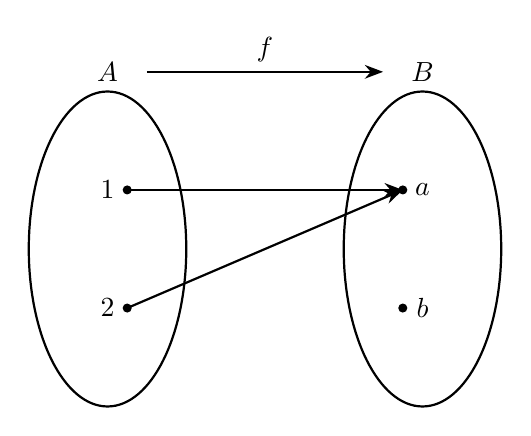
\begin{tikzpicture}
	% Draw the sets A and B
	\draw[thick] (-2,0) ellipse (1 and 2);
	\draw[thick] (2,0) ellipse (1 and 2);
	
	% Labels for sets
	\node at (-2, 2.25) {$A$};
	\node at (2, 2.25) {$B$};
	
	% Draw the arrows representing the function
	\draw[-Stealth, thick] (-1.5, 2.25) -- (1.5,2.25) node[midway, above] {$f$};
	
	\node at (-2, .75) {$1$};
	\node at (-2, -.75) {$2$};
	\draw[fill] (-1.75,.75) circle (.05);
	\draw[fill] (-1.75,-.75) circle (.05);
	
	\node at (2, .75) {$a$};
	\node at (2, -.75) {$b$};
	\draw[fill] (1.75,.75) circle (.05);
	\draw[fill] (1.75,-.75) circle (.05);
	
	\draw[-Stealth, thick] (-1.75, .75) -- (1.75, .75);
	\draw[-Stealth, thick] (-1.75, -.75) -- (1.75, .75);
\end{tikzpicture}

	\end{center}
	\begin{enumerate}[(1)]
		\item Let $B_1=\set{b}\subseteq B$. Then $f^{-1}[B_1]=\varnothing$ and so \[
		f[f^{-1}[B]]=f[\varnothing]=\varnothing\neq \set{b}=B_1.
		\]
		\item Let $A_1=\set{1}\subseteq A$. Then $f[A_1]=f[\set{1}]=\set{a}$ and so \[
		f^{-1}[f[A_1]]=f^{-1}[\set{a}]=\set{1,2}\neq \set{1}=A_1.
		\]
	\end{enumerate}
\end{example*}
\vfill
\defbox[Injection and Surjection]{\begin{definition*}
	Let $f:A\to B$ is a function from $A$ to $B$. \begin{itemize}
		\item  A function $f$ is \hl{\textbf{an injection}} or \hl{\textbf{injective}} (or \hl{\textbf{one-to-one}}) if and only if \[
		\boxed{\forall a_1,a_2\in A:[f(a_1)=f(a_2)\implies a_1=a_2].}
		\] That is, an \textbf{injection} is a mapping such that the output uniquely determines its input.
		\item A function $f$ is \hl{\textbf{a surjection}} or \hl{\textbf{surjective}} (or \hl{\textbf{onto}}) if and only if \[
		\boxed{\forall b\in B:[\exists a \in A\ \text{such that}\ f(a)=b].}
		\] That is, a \textbf{surjection} is a mapping such that every element of $B$ is related to by some element of $A$.
	\end{itemize}
\end{definition*}}
\begin{remark*}
	A function $f$ is \textbf{bijective} if and only if $f$ is both injective and surjective.
	\begin{itemize}
		\item $f$ is \hl{\textbf{a bijection}} (or \hl{\textbf{bijective}}).
		\item $f$ is \hl{\textbf{one-to-one and onto}} (or \hl{\textbf{a one-to-one correspondence}}).
	\end{itemize}
\end{remark*}

\defbox[Composition of Functions]{\begin{definition*}
		Let $f_1:A\to B$ and $f_2:B\to C$ be functions such that $\text{Cdm}(f_1)=B=\text{Dom}(f_2)$. The \hl{\textbf{composition}} $f_2\circ f_1$ is defined as: \[
		(f_2\circ f_1)(a):= f_2(f_1(a)).
		\] for all $a\in A$.
\end{definition*}}
%\begin{remark*}
%\ \begin{itemize}
%	\item $f_2\circ f_1=\set{(a,c)\in A\times C: (f_1(a), c)\in f_2}=\set{(a,c)\in A\times C: c=f_2(f_1(a))}$.
%	\item $f_2\circ f_1=\set{(a,c)\in A\times C: \exists b\in f_2\ \text{s.t.}\ f_1(a)=b\land f_2(b)=c}$.
%\end{itemize}
%\end{remark*}
\begin{note}[Diagram]
	\ \begin{figure}[h!]
		\centering
		\begin{tikzcd}
	A \arrow[rrr, "f_1"] \arrow[rrrddd, "f_2\circ f_1"', dashed] &  &  & B \arrow[ddd, "f_2"] \\
	&  &  &                        \\
	&  &  &                        \\
	&  &  & C                   
\end{tikzcd}

		\caption{Diagram of $f_2\circ f_1$.}
	\end{figure}
\end{note}
\newpage
\begin{note}[Illustration]
	\ \begin{figure}[h!]\centering
		\adjustbox{scale=.9}{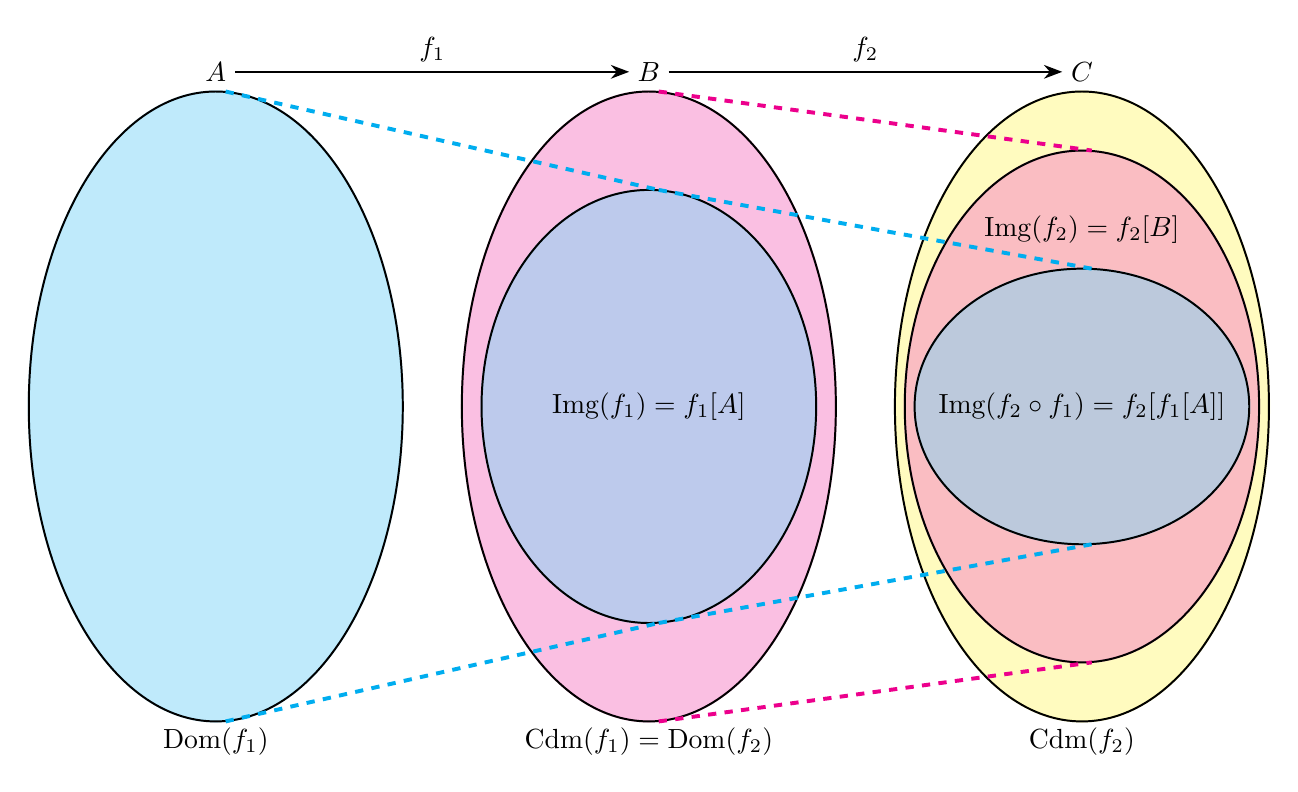
\begin{tikzpicture}[scale=.5]
	\def \x {11};
	\def \ellmajor {8};
	\def \ellminor {2.75};
	% Draw the sets A, B and C
	\filldraw[thick, cyan!50, opacity=.5] (-\x,0) ellipse (4.75 and \ellmajor);
	\draw[thick, line width = .25mm] (-\x,0) ellipse (4.75 and \ellmajor);
	\filldraw[thick, magenta!50, opacity=.5] (0,0) ellipse (4.75 and \ellmajor);
	\draw[thick, line width = .25mm] (0,0) ellipse (4.75 and \ellmajor);
	\filldraw[thick, yellow!50, opacity=.5] (\x,0) ellipse (4.75 and \ellmajor);
	\draw[thick, line width = .25mm] (\x,0) ellipse (4.75 and \ellmajor);
	
	\filldraw[thick, cyan!50, opacity=.5] (0,0) ellipse (4.25 and 5.5);
	\draw[thick, line width = .25mm] (0,0) ellipse (4.25 and 5.5);
	
	\filldraw[thick, magenta!50, opacity=.5] (\x,0) ellipse (4.5 and 6.5);
	\draw[thick, line width = .25mm] (\x,0) ellipse (4.5 and 6.5);
	\filldraw[thick, cyan!50, opacity=.5] (\x,0) ellipse (4.25 and 3.5);
	\draw[thick, line width = .25mm] (\x,0) ellipse (4.25 and 3.5);
	
	% Draw the arrows representing the function
	\draw[-Stealth, thick] (-\x + .5, 8.5) -- (-.5, 8.5) node[midway, above] {$f_1$};
	\draw[-Stealth, thick] (.5, 8.5) -- (\x - .5, 8.5) node[midway, above] {$f_2$};
	
	% Labels for sets
	\node at (-\x, 8.5) {$A$};
	\node at (0, 8.5) {$B$};
	\node at (\x, 8.5) {$C$};
	
	\node at (0, 0) {$\img{f_1}=f_1[A]$};
	\draw[dashed, thick, line width= .5mm, color=cyan] (-\x + .25, \ellmajor) -- (.25, 5.5);
	\draw[dashed, thick, line width= .5mm, color=cyan] (-\x + .25, -\ellmajor) -- (.25, -5.5);
	
	\node at (\x, 4.5) {$\img{f_2}=f_2[B]$};
	\draw[dashed, thick, line width= .5mm, color=magenta] (0.25, \ellmajor) -- (\x + .25, 6.5);
	\draw[dashed, thick, line width= .5mm, color=magenta] (0.25, -\ellmajor) -- (\x + .25, -6.5);
	
	\node at (\x, 0) {$\img{f_2\circ f_1}=f_2[f_1[A]]$};
	\draw[dashed, thick, line width= .5mm, color=cyan] (0.25, 5.5) -- (\x + .25, 3.5);
	\draw[dashed, thick, line width= .5mm, color=cyan] (0.25, -5.5) -- (\x + .25, -3.5);
	
	\node at (-\x, -8.5) {$\text{Dom}(f_1)$};
	\node at (0, -8.5) {$\text{Cdm}(f_1)=\text{Dom}(f_2)$};
	\node at (\x, -8.5) {$\text{Cdm}(f_2)$};
\end{tikzpicture}
}
		\caption{Illustration of $f_2\circ f_1$}
	\end{figure}
\end{note}
\vfill
\begin{remark*}
	The composition is associative. For any \( f, g, h \in G \), $
	(f \circ g) \circ h = f \circ (g \circ h) $.
	\begin{figure}[h!]\centering
		\adjustbox{scale=.9}{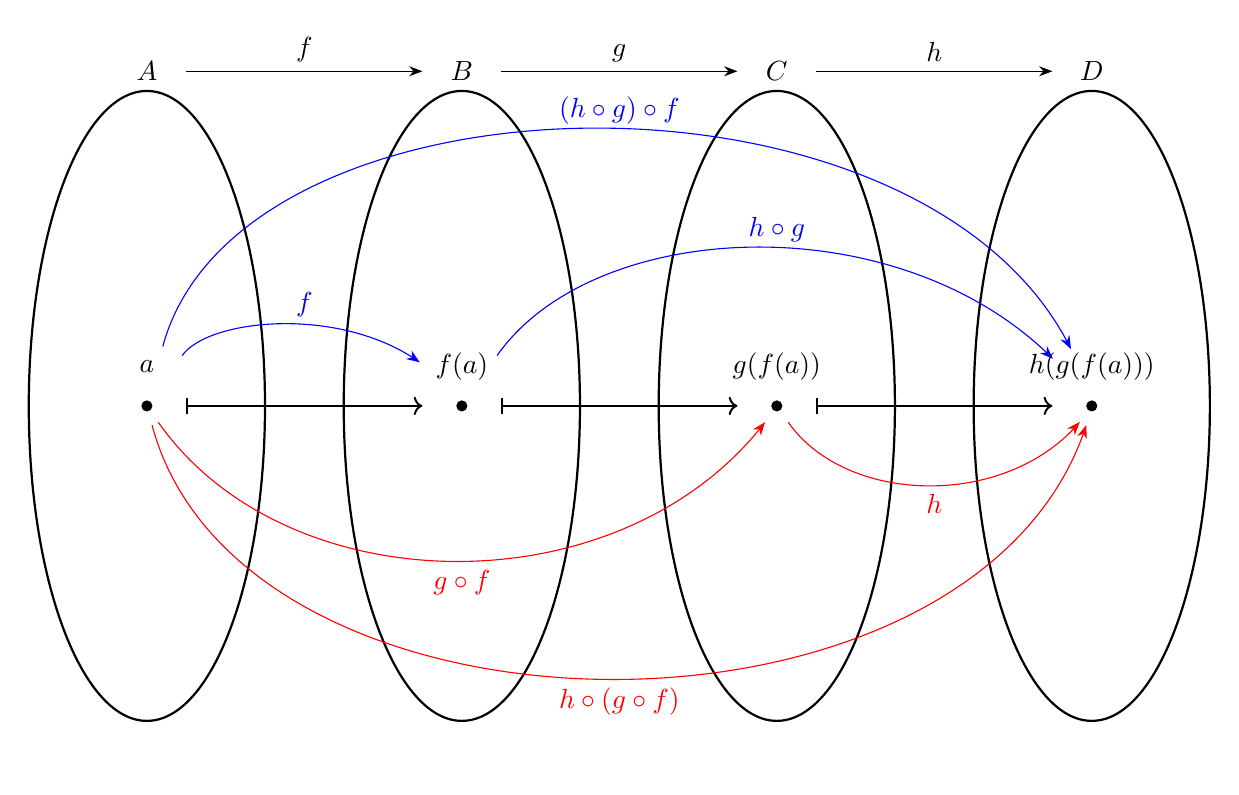
\begin{tikzpicture}
	\draw[thick] (-6,0) ellipse (1.5 and 4);
	\draw[thick] (-2,0) ellipse (1.5 and 4);
	\draw[thick] (2,0) ellipse (1.5 and 4);
	\draw[thick] (6,0) ellipse (1.5 and 4);
	
	\node at (-6, 4.25) {$A$};
	\node at (-2, 4.25) {$B$};
	\node at (2, 4.25) {$C$};
	\node at (6, 4.25) {$D$};
	
	\draw[-Stealth] (-5.5, 4.25) -- (-2.5, 4.25) node[midway, above] {$f$};
	\draw[-Stealth] (-1.5, 4.25) -- (1.5, 4.25) node[midway, above] {$g$};
	\draw[-Stealth] (2.5, 4.25) -- (5.5, 4.25) node[midway, above] {$h$};
	\draw[|->, line width=.25mm] (-5.5, 0) -- (-2.5, 0);
	\draw[|->, line width=.25mm] (-1.5, 0) -- (1.5, 0);
	\draw[|->, line width=.25mm] (2.5, 0) -- (5.5, 0);
	
	\node[fill, circle, inner sep=0.05cm] at (-6,0) (A) {};
	\node[fill, circle, inner sep=0.05cm] at (-2,0) (B) {};
	\node[fill, circle, inner sep=0.05cm] at (2,0) (C) {};
	\node[fill, circle, inner sep=0.05cm] at (6,0) (D) {};
	\node (A2) at (-6, 0.5) {$a$};
	\node (B2) at (-2, 0.5) {$f(a)$};
	\node (C2) at (2, 0.5) {$g(f(a))$};
	\node (D2) at (6, 0.5) {$h(g(f(a)))$};
	
	\draw[-Stealth, bend right=55pt, shorten <= 5pt, shorten >= 5pt, red] (A) to node[midway,below] {$g\circ f$} (C);
	\draw[-Stealth, bend right=55pt, shorten <= 5pt, shorten >= 5pt, red] (C) to node[midway,below] {$h$} (D);
	\draw[-Stealth, bend right=75pt, shorten <= 5pt, shorten >= 5pt, red] (A) to node[midway,below] {$h\circ(g\circ f)$} (D);
	
	\draw[-Stealth, bend left=75pt, shorten <= 20pt, shorten >= 20pt, blue] (A) to node[midway,above] {$(h\circ g)\circ f$} (D);
	\draw[-Stealth, bend left=55pt, shorten <= 20pt, shorten >= 20pt, blue] (A) to node[midway,above] {$f$} (B);
	\draw[-Stealth, bend left=55pt, shorten <= 20pt, shorten >= 20pt, blue] (B) to node[midway,above] {$h\circ g$} (D);
\end{tikzpicture}
}
		\caption{Associativity of Composition.}
	\end{figure}
\end{remark*}
\newpage
\thmbox[]{\begin{theorem}
	Let $A$ and $B$ are sets. Let $f:A\to B$ be a function.
	\begin{enumerate}[(1)]
		\item $f$ is one-to-one if and only if there exists the function $g:B\to A$ such that $g\circ f =\textnormal{id}_A$.
		\item $f$ is onto if and only if there exists the function $g:B\to A$ such that $f\circ g =\textnormal{id}_B$.
	\end{enumerate}
\end{theorem}}
\begin{remark*}
	\ \begin{center}
		(1) % https://tikzcd.yichuanshen.de/#N4Igdg9gJgpgziAXAbVABwnAlgFyxMJZABgBpiBdUkANwEMAbAVxiRAEEQBfU9TXfIRQAmclVqMWbAELdeIDNjwEiAFjHV6zVog7dxMKAHN4RUADMAThAC2SMiBwQkARk2SdIc3IvW7iN0dnRFEJbTYjHy8-e2onJFCAIxgwKCQAWgBmBwY6ZIYABX5lIRBLLCMACxwQd3DdIwAdRoBjLEsWgAJzToBeTuacGAAPHEhLG0ZgLCguAH1OLgouIA
		\begin{tikzcd}
			A \arrow[rr, "\textcolor{red}{f}"] \arrow[rrrr, "\textcolor{green!50!black}{g}\circ \textcolor{red}{f} = \textnormal{id}_A"', bend right] &  & B \arrow[rr, "\exists\textcolor{green!50!black}{g}"] &  & A
		\end{tikzcd}\hspace{50pt} (2) % https://tikzcd.yichuanshen.de/#N4Igdg9gJgpgziAXAbVABwnAlgFyxMJZABgBpiBdUkANwEMAbAVxiRACEQBfU9TXfIRQAmclVqMWbAILdeIDNjwEiAFjHV6zVog7dxMKAHN4RUADMAThAC2SMiBwQkARk2SdII3IvW7iN0dnRFEJbTZzHxArW3tqJyRQgCMYMCgkAFoAZgcGOhSGAAV+ZSEQSywjAAscEHdw3XMAHSaAYyxLVoACIy6AXi6WnBgADxxISxtGYCwoLgB9Ti4KLiA
		\begin{tikzcd}
		B \arrow[rr, "\exists\textcolor{green!50!black}{g}"] \arrow[rrrr, "\textcolor{red}{f}\circ\textcolor{green!50!black}{g} = \textnormal{id}_B"', bend right] &  & A \arrow[rr, "\textcolor{red}{f}"] &  & B
	\end{tikzcd}
	\end{center}
\end{remark*}
\begin{proof}
\begin{enumerate}[(1)]
	\item \begin{itemize}
		\item[($\Rightarrow$)] Assume that $f:A\to B$ is injective. We need to construct a function $g:B\to A$ such that $g\circ f=\textnormal{id}_A$.
		\begin{center}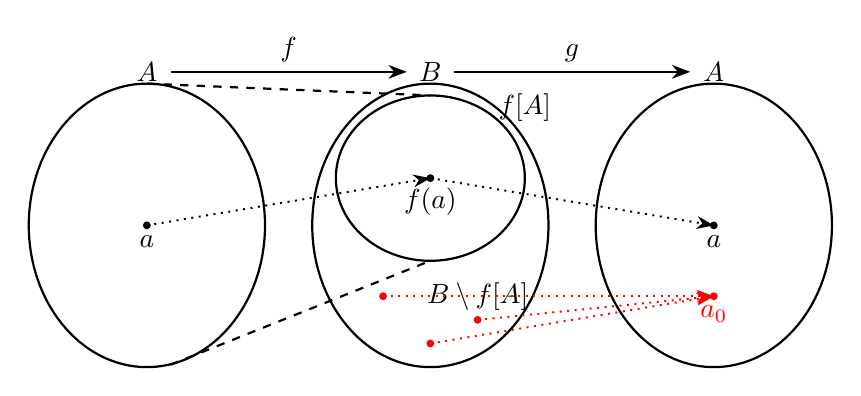
\begin{tikzpicture}[>=Stealth, scale=.6]
		% Draw the sets A, B and C
		\draw[thick] (-6,0) ellipse (2.5 and 3);
		\draw[thick] (0,0) ellipse (2.5 and 3);
		\draw[thick] (6,0) ellipse (2.5 and 3);
		
		\draw[thick] (0,1) ellipse (2 and 1.75);
		
		% Draw the arrows representing the function
		\draw[-Stealth, thick] (-5.5, 3.25) -- (-.5,3.25) node[midway, above] {$f$};
		\draw[-Stealth, thick] (.5, 3.25) -- (5.5,3.25) node[midway, above] {$g$};
		
		% Labels for sets
		\node at (-6, 3.25) {$A$};
		\node at (0, 3.25) {$B$};
		\node at (6, 3.25) {$A$};
		
		\node at (2, 2.5) {$f[A]$};
		\draw[dashed, thick] (-6, 3) -- (0,2.75);
		\draw[dashed, thick] (-5.5, -2.95) -- (0,-.75);
		\node at (1, -1.5) {$B\setminus f[A]$};
		
		\filldraw (-6,0) circle (2pt) node[below] {$a$};
		\draw[->, dotted, line width = .25mm] (-6, 0) -- (0,1);
		\filldraw (0,1) circle (2pt) node[below] {$f(a)$};
		\draw[->, dotted, line width = .25mm] (0, 1) -- (6,0);
		\filldraw (6,0) circle (2pt) node[below] {$a$};
		
		\filldraw[red] (0,-2.5) circle (2pt) ;
		\filldraw[red] (-1,-1.5) circle (2pt) ;
		\filldraw[red] (1,-2) circle (2pt) ;
		\filldraw[red] (6,-1.5) circle (2pt) node[below] {$a_0$};
		\draw[->, dotted, red, line width = .25mm] (0, -2.5) -- (6,-1.5);
		\draw[->, dotted, red, line width = .25mm] (-1, -1.5) -- (6,-1.5);
		\draw[->, dotted, red, line width = .25mm] (1, -2) -- (6,-1.5);
		\end{tikzpicture}
	\end{center}
	We define a function $g:B\to A$ given by \[
	g(b)=\begin{cases}
			a &\text{if}\ \exists! a\in A\ \text{such that}\ f(a)=b \\
			a_0 &\text{if}\ b\notin f[A]
	\end{cases}
	\] for all $b\in B$, where $a_0\in A$ is an arbitrary element of $A$. Since $f$ is one-to-one, $g$ is well-defined.
	For any $a\in A$, we have $f(a)\in B$. By the definition of $g$, we obtain $g(f(a))=a. $ Thus, \[
	(g\circ f)(a)=g(f(a))=a=\text{id}_A(a)
	\] for all $a\in A$.
	\vfill
	\item[($\Leftarrow$)] \textcolor{gray!30!white}{Assume that there exists $g:B\to A$ such that $g\circ f=\text{id}_A$. Suppose that $f(a_1)=f(a_2)$ for any $a_1,a_2\in A$. Then \begin{align*}
		f(a_1)=f(a_2) &\implies g(f(a_1))=g(f(a_2))\quad\text{by def. of a function}\\
		&\implies a_1=a_2\quad\text{by assumption}\ g\circ f=\text{id}_A.
	\end{align*}}
	\end{itemize}
	\item \begin{itemize}
		\item[($\Rightarrow$)] Assume $f:A\to B$ is surjective. Then, for every $b\in B$, there exists at least one $a\in A$ such that $f(a)=b$. We need to construct a function $g:B\to A$ such that $f\circ g=\textnormal{id}_B$, \ie, $f(g(b))=b$ for every $b\in B$.
		\begin{center}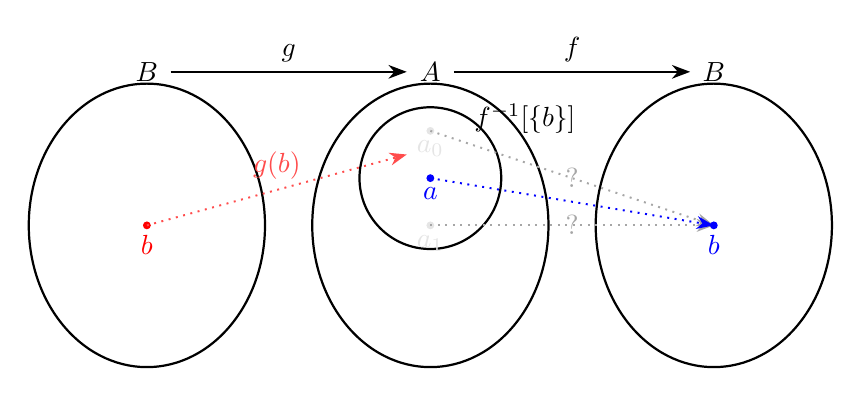
\begin{tikzpicture}[>=Stealth, scale=.6]
				% Draw the sets A, B and C
				\draw[thick] (-6,0) ellipse (2.5 and 3);
				\draw[thick] (0,0) ellipse (2.5 and 3);
				\draw[thick] (6,0) ellipse (2.5 and 3);
				
				\draw[thick] (0,1) ellipse (1.5 and 1.5);
				
				% Draw the arrows representing the function
				\draw[-Stealth, thick] (-5.5, 3.25) -- (-.5,3.25) node[midway, above] {$g$};
				\draw[-Stealth, thick] (.5, 3.25) -- (5.5,3.25) node[midway, above] {$f$};
				
				% Labels for sets
				\node at (-6, 3.25) {$B$};
				\node at (0, 3.25) {$A$};
				\node at (6, 3.25) {$B$};
				
				\node at (2, 2.25) {$f^{-1}[\set{b}]$};
				
				\filldraw[gray!20!white] (0,2) circle (2pt) node[below] {$a_0$};
				\filldraw[gray!20!white] (0,0) circle (2pt) node[below] {$a_1$};
				\draw[->, dotted, gray!70!white, line width = .25mm] (0, 2) -- (6, 0) node[midway] {?};
				\draw[->, dotted, gray!70!white, line width = .25mm] (0, 0) -- (6, 0) node[midway] {?};
				
				\filldraw[blue] (0,1) circle (2pt) node[below] {$a$};
				\filldraw[blue] (6,0) circle (2pt) node[below] {$b$};
				\draw[->, dotted, blue, line width = .25mm] (0, 1) -- (6, 0);
				
				\filldraw[red] (-6,0) circle (2pt) node[below] {$b$};
				\draw[->, dotted, red!70!white, line width = .25mm] (-6, 0) -- (-.5, 1.5) node[midway, above] {$g(b)$};
			\end{tikzpicture}
		\end{center}
		The \textbf{Axiom of Choice}\footnote{\textcolor{gray!70!white}{Here, $\mathbb{S}=\set{f^{-1}[\set{b}]\subseteq A:b\in B}$ and $\bigcup\mathbb{S}=\bigcup_{b\in B}f^{-1}[\set{b}]=A$. That is, there is a choice function $F:\mathcal{P}(A)\setminus\set{\emptyset}\to A$.}} allows us to define $g:B\to A$ given by \[
		g(b)=a\in f^{-1}[\set{b}]
		\] for each $b\in B$. Thus, \begin{align*}
			(f\circ g)(b) &= f(g(b))&\text{by def. of composition} \\
			&=f(a) &\text{by def. of $g$} \\
			&=b &\text{by assumption} \\
			&=\text{id}_B(b)
		\end{align*} for all $b\in B$. That is, $f\circ g=\text{id}_B$. Without the Axiom of Choice, we cannot always guarantee the existence of such a selection function, especially when the sets $f^{-1}[\set{b}]$ are uncountable.
		\vspace{12pt}
		\item[($\Leftarrow$)] \textcolor{gray!30!white}{Assume that there exists $g:B\to A$ such that $f\circ g=\text{id}_B$. Let $b\in B$. Since $f\circ g=\text{id}_B$, we have $f(g(b))=\text{id}_B(b)=b$. Thus, for every $b\in B$, \[
		\exists a=g(b)\in A\quad\text{such that}\quad f(a)=f(g(b))=b.
		\]}
	\end{itemize}
\end{enumerate}
\end{proof}

\newpage
\begin{note}[Axiom of Choice]
	Let $\mathbb{S}$ be a set of non-empty sets. \begin{center}
		``It is always possible to construct a choice function \\ that selects a one element from each member of the set.''
	\end{center} \textcolor{gray!30!white}{Formally, \[
	\forall\mathbb{S}:\left[\varnothing\notin \mathbb{S}\implies\exists\left(f:\mathbb{S}\to\bigcup\mathbb{S}\right)\ \text{s.t.}\ \forall X\in\mathbb{S}:[f(X)\in X]\right].
	\]}
	\vspace{24pt} \\
	\noindent For example, let $\mathbb{S}=\set{A,B,C,\dots}$ and $\bigcup\mathbb{S}=A\cup B\cup C\cup\cdots$.
	\begin{center}
	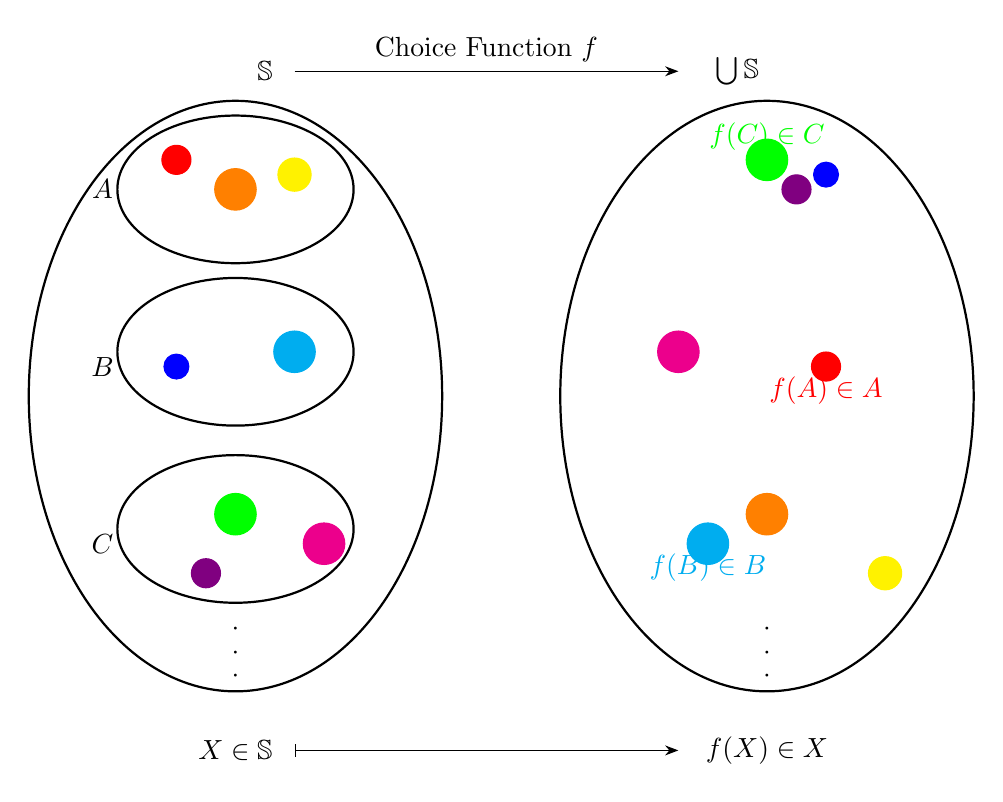
\begin{tikzpicture}[>=Stealth, scale=.75]
		\draw[thick] (-4.5,0) ellipse (3.5 and 5);
		\draw[thick] (4.5,0) ellipse (3.5 and 5);
		\node at (-4, 5.5) {$\mathbb{S}$};
		\node at (4, 5.5) {$\bigcup\mathbb{S}$};
		\draw[->] (-3.5, 5.5) -- (3, 5.5) node[midway, above] {Choice Function $f$};
		
		\draw[thick] (-4.5,3.5) ellipse (2 and 1.25); \node at (-6.75, 3.5) {$A$};
		\draw[thick] (-4.5,.75) ellipse (2 and 1.25); \node at (-6.75, .5) {$B$};
		\draw[thick] (-4.5,-2.25) ellipse (2 and 1.25); \node at (-6.75, -2.5) {$C$};
		\node at (-4.5, -3.95) {$\cdot$};
		\node at (-4.5, -4.35) {$\cdot$};
		\node at (-4.5, -4.75) {$\cdot$};
		
		% Elements of A
		\filldraw[red] (-5.5, 4) circle (7pt);
		\filldraw[orange] (-4.5, 3.5) circle (10pt);
		\filldraw[yellow] (-3.5, 3.75) circle (8pt);
		
		% Elements of B
		\filldraw[blue] (-5.5, .5) circle (6pt);
		\filldraw[cyan] (-3.5, .75) circle (10pt);
		
		% Elements of C
		\filldraw[green] (-4.5, -2) circle (10pt);
		\filldraw[violet] (-5, -3) circle (7pt);
		\filldraw[magenta] (-3, -2.5) circle (10pt);
		
		% Elements of Codomain
		\filldraw[red] (5.5, .5) circle (7pt) node[below] {$f(A)\in A$};
		\filldraw[orange] (4.5, -2) circle (10pt);
		\filldraw[yellow] (6.5, -3) circle (8pt);
		\filldraw[blue] (5.5, 3.75) circle (6pt);
		\filldraw[cyan] (3.5, -2.5) circle (10pt) node[below] {$f(B)\in B$};
		\filldraw[green] (4.5, 4) circle (10pt) node[above] {$f(C)\in C$};
		\filldraw[violet] (5, 3.5) circle (7pt);
		\filldraw[magenta] (3, .75) circle (10pt);
		\node at (4.5, -3.95) {$\cdot$};
		\node at (4.5, -4.35) {$\cdot$};
		\node at (4.5, -4.75) {$\cdot$};
		
		% Mapsto
		\node at (-4.5, -6) {$X\in\mathbb{S}$};
		\node at (4.5, -6) {$f(X)\in X$};
		\draw[|->] (-3.5, -6) -- (3, -6);
	\end{tikzpicture}
\end{center}
\end{note}

\vfill
\begin{thebibliography}{9}
	\bibitem{set_thery_a}
	수학의 즐거움, Enjoying Math. ``수학 공부, 기초부터 대학원 수학까지, 1. 집합론 기초 (a).'' YouTube Video, 30:55. Published 
	September 05, 2019. URL: \url{https://www.youtube.com/watch?v=9HUk8zays2E&list=PL4m4z_pFWq2pLwFsWf0KJX_uMNo-jktN5&index=132}.
	
	\bibitem{set_thery_b}
	수학의 즐거움, Enjoying Math. ``수학 공부, 기초부터 대학원 수학까지, 2. 집합론 기초 (b).'' YouTube Video, 29:06. Published 
	September 05, 2019. URL: \url{https://www.youtube.com/watch?v=k53Sr9Q9NR8&list=PL4m4z_pFWq2pLwFsWf0KJX_uMNo-jktN5&index=133}.
\end{thebibliography}

\end{document}
